\documentclass[a4paper]{article}
\usepackage[T1]{fontenc}
\usepackage[utf8]{inputenc}
\usepackage{tocloft,siunitx,amsmath,graphicx,subcaption,float}
\usepackage[top=3cm,left=3cm,right=3cm]{geometry}
\graphicspath{{img/}}
\renewcommand\cftsecfont{\normalfont}
\renewcommand\cftsecpagefont{\normalfont}
\renewcommand{\cftsecleader}{\cftdotfill{\cftsecdotsep}}
\renewcommand\cftsecdotsep{\cftdot}
\renewcommand\cftsubsecdotsep{\cftdot}
\renewcommand\cftsubsubsecdotsep{\cftdot}
\title{Lab 1}
%\author{
%    Sebastián Nava López\\
%    \and
%    Ericka Sabrina Pensamiento R.\\
%    \and
%    Salvador Palos Gil
%}
\captionsetup[subfigure]{justification=raggedright}
\begin{document}
\begin{titlepage}
    \centering
    {\Huge Instituto Politécnicno Nacional}\\[3ex]
    {\huge Escuela Superior de Cómputo}\\[8ex]
    {\huge Fundamental Circuit Analysis}\\[12ex]
    {\Large Lab 1: Ohmeter,Voltmeter and Ampmeter usage}\\[20ex]
    {\Large Group: 1CV7 Team: 7 \\[8ex]
    Sebastian Nava López\\[4ex]
    Sabrina Erika Pensamiento Robledo\\[4ex]
    Salvador Palos Gil\\[18ex]
    }
    \large{Elaboration: February 27,2018\hspace{8em} Due date: March 6,2018}
    

\end{titlepage}
\tableofcontents
\newpage
\section{Introduction}
In the realm of electrical engineering, we tend to work with conductive materials which have very little resistance to the pass of an electric current, this physical property of materials is called Electrical Resistance and its unit is the ohm (\si{\ohm}). We can also measure the rate at which electrical charges are flowing through the material in relation to the time at a certain point, this is called Electric Current and it is measured in ampere (A). Finally, conductive materials have another physical property called Electronic Potential or Voltage, this is described as the energy or work required to move a unit of charge between two points and it is measured in volts (V). 

These three elements are used and/or required to make a proper functioning electric circuit which we can define, to this specific context, as an electrical connection than can serve many, many uses.

All those properties can be measured in a circuit using the appropriate instruments. This instruments can be direct-reading(analog) or digital, the main difference between this two resides in the way they display the information; the first uses the deflection of a needle while the other uses a digital display to show the variable values. The ammeter is the instrument used to measure current, it uses a pair of terminals called probes which are usually colored with red and black. When we need to measure the current in a circuit, we need to open the circuit in the desired point, then we connect both probes in series in said point, then the ammeter will measure the current going from the red to the black probe. 

The voltmeter is used to measure voltage and it works similarly to the ammeter, but instead of connecting the probes in series, we need to connect the probes in parallel to the segment of the circuit that we want to measure. 

The ohmmeter measures the resistance and, like the ammeter and voltmeter, also has a pair of probes. In order to get the resistance value, we put the probes in the segment we want to measure, then, if there is continuity between the leads and the circuit is not shorted, it will show the resistance value. It is worth noting that, to make the ohmmeter work properly, the circuit that is being measured must be de-energized. Usually, these three instruments come in a single unit called multimeter. This three meters are very useful when we want to analyze circuits as well as when we want to design new ones.

\newpage
\section{Development}
\subsection{Ohmmeter Usage}
In the first part of the experiment we calculated the resistance value of all the resistors using the color code, then we connected the resistors into the breadboard, and,with the resistance function of the multimeter, measured the resistance value for each resistor 12 times.
\subsubsection{Calculations}
In $R_1$, given that the first strip is green(digit 5),the next is blue(digit 6),and the third is brown(digit 1) ,the value of resistance is:
\[\SI{56e1}=\SI{560}{\ohm}\]
In R2, given that the first strip is brown(digit 1),the next is black(digit 0),and the third is red(digit 2) ,the value of resistance is:
\[\SI{10e2}=\SI{1000}{\ohm}\]
In R3, given that the first strip is orange(digit 3),the next is orange(digit 3),and the third is brown(digit 1) ,the value of resistance is:
\[\SI{33e1}=\SI{330}{\ohm}\]
In R4, given that the first strip is blue(digit 6),the next is grey(digit 8),and the third is brown(digit 1) ,the value of resistance is:
\[\SI{68e1}=\SI{680}{\ohm}\]
\subsubsection{Measurements}
\begin{center}
\begin{tabular}{|c|c|c|}
\hline
Resistor & Digital Ohmmeter & Color code values\\ \hline
$R_1$ & $\SI{549}{\ohm}$ & $\SI{56e1}{\ohm}=\SI{560}{\ohm}$ \\ \hline
$R_2$ & $\SI{987}{\ohm}$ & $\SI{10e2}{\ohm}=\SI{1}{\kilo\ohm}$ \\ \hline
$R_3$ & $\SI{325}{\ohm}$ & $\SI{33e1}{\ohm}=\SI{330}{\ohm}$ \\ \hline
$R_4$ & $\SI{671}{\ohm}$ & $\SI{68e1}{\ohm}=\SI{680}{\ohm}$ \\ \hline
\end{tabular}
\end{center}
\subsubsection{Simulations}
\begin{figure}[H]
\begin{subfigure}{0.48\textwidth}
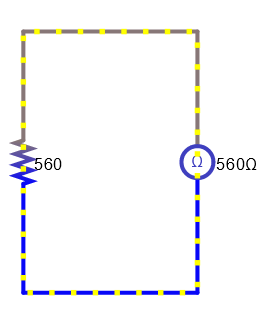
\includegraphics[width=\linewidth,height=7.4cm]{ohm_560}
\caption{$\SI{560}{\ohm}$ Resistor ($R_1$)}
\end{subfigure}
\begin{subfigure}{0.48\textwidth}
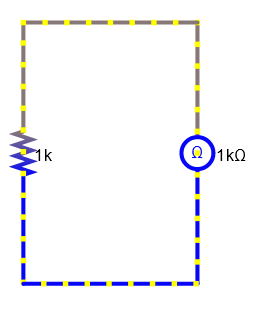
\includegraphics[width=\linewidth,height=7.4cm]{ohm_1k}
\caption{$\SI{1}{\kilo\ohm}$ Resistor ($R_2$)}
\end{subfigure}
\caption{Ohmmeter simulation for $R_1$ and $R_2$}
\label{fig:1}
\end{figure}

\begin{figure}[H]
\begin{subfigure}{0.48\textwidth}
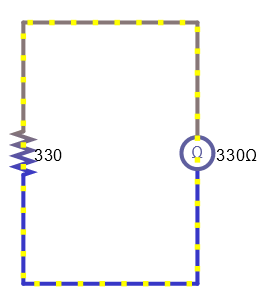
\includegraphics[width=\linewidth]{ohm_330}
\caption{$\SI{560}{\ohm}$ Resistor ($R_1$)}
\end{subfigure}
\begin{subfigure}{0.48\textwidth}
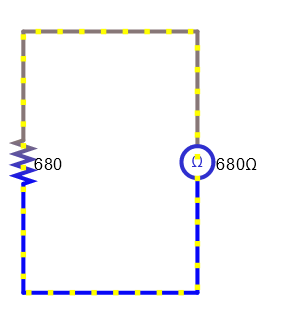
\includegraphics[width=\linewidth]{ohm_680}
\caption{$\SI{1}{\kilo\ohm}$ Resistor ($R_2$)}
\end{subfigure}
\caption{Ohmmeter simulation for $R_1$ and $R_2$}
\label{fig:2}
\end{figure}
\subsection{Voltmeter usage}
In the second part of the experiment, using the \SI{1}{\kilo\ohm} and the \SI{330}{\ohm} resistors connected in series in the breadboard and powered by a voltage supply set at \SI{1}{\volt} , we measured the voltage in each resistor and in the equivalent resistor twelve times, augmenting \SI{1}{\volt} of the value of the voltage supply each time. 
\subsubsection{Calculations}
Using KVL(Kirchhoff’s Voltage Law) we know that 
\[-V+VR_1+VR_2=0\]
Given that the circuit is connected in series, the current $i$ is the same for both resistors
\begin{align*}
V&=iR_1+iR_2\\
V&=i(R_1+R_2)
\end{align*}
Isolating the current $i$:
\[i=\frac{V}{R_1+R_2}\]
Also, if the circuit is connected in series, the voltage for each resistor is different, so :
\begin{align*}
V_1&=iR_1\\ 
V_2&=iR_2
\end{align*}
Plugging the value of $i$ in $V_1$ and $V_2$, we have:
\begin{align*}
V_1&=\frac{R_1V}{R_1+R_2}\\ 
V_2&=\frac{R_2V}{R_1+R_2}
\end{align*}
Finally, if we want the voltage in the equivalent resistor, is the same value as the one specified in the voltage supply.
For each voltage we have:\\
%1V
$E=\SI{1}{\volt}$
\[V_1=\frac{\SI{1}{\volt}\cdot\SI{1}{\kilo\ohm}}{\SI{1}{\kilo\ohm}+\SI{330}{\ohm}}=\SI{0.752}{\volt}
\qquad
V_2=\frac{\SI{1}{\volt}\cdot\SI{330}{\ohm}}{\SI{1}{\kilo\ohm}+\SI{330}{\ohm}}=\SI{0.248}{\volt}
\qquad
V_{t}=\SI{1}{\volt}
\]
%2V
$E=\SI{2}{\volt}$
\[V_1=\frac{\SI{2}{\volt}\cdot\SI{1}{\kilo\ohm}}{\SI{1}{\kilo\ohm}+\SI{330}{\ohm}}=\SI{1.504}{\volt}
\qquad
V_2=\frac{\SI{2}{\volt}\cdot\SI{330}{\ohm}}{\SI{1}{\kilo\ohm}+\SI{330}{\ohm}}=\SI{0.496}{\volt}
\qquad
V_{t}=\SI{2}{\volt}
\]
%3V
$E=\SI{3}{\volt}$
\[V_1=\frac{\SI{3}{\volt}\cdot\SI{1}{\kilo\ohm}}{\SI{1}{\kilo\ohm}+\SI{330}{\ohm}}=\SI{2.255}{\volt}
\qquad
V_2=\frac{\SI{3}{\volt}\cdot\SI{330}{\ohm}}{\SI{1}{\kilo\ohm}+\SI{330}{\ohm}}=\SI{0.744}{\volt}
\qquad
V_{t}=\SI{3}{\volt}
\]
%4V
$E=\SI{4}{\volt}$
\[V_1=\frac{\SI{4}{\volt}\cdot\SI{1}{\kilo\ohm}}{\SI{1}{\kilo\ohm}+\SI{330}{\ohm}}=\SI{3.01}{\volt}
\qquad
V_2=\frac{\SI{4}{\volt}\cdot\SI{330}{\ohm}}{\SI{1}{\kilo\ohm}+\SI{330}{\ohm}}=\SI{0.992}{\volt}
\qquad
V_{t}=\SI{4}{\volt}
\]
%5V
$E=\SI{5}{\volt}$
\[V_1=\frac{\SI{5}{\volt}\cdot\SI{1}{\kilo\ohm}}{\SI{1}{\kilo\ohm}+\SI{330}{\ohm}}=\SI{3.759}{\volt}
\qquad
V_2=\frac{\SI{5}{\volt}\cdot\SI{330}{\ohm}}{\SI{1}{\kilo\ohm}+\SI{330}{\ohm}}=\SI{1.241}{\volt}
\qquad
V_{t}=\SI{5}{\volt}\]
%6V
$E=\SI{6}{\volt}$
\[V_1=\frac{\SI{6}{\volt}\cdot\SI{1}{\kilo\ohm}}{\SI{1}{\kilo\ohm}+\SI{330}{\ohm}}=\SI{4.511}{\volt}
\qquad
V_2=\frac{\SI{6}{\volt}\cdot\SI{330}{\ohm}}{\SI{1}{\kilo\ohm}+\SI{330}{\ohm}}=\SI{1.489}{\volt}
\qquad
V_{t}=\SI{6}{\volt}
\]
%7V
$E=\SI{7}{\volt}$
\[V_1=\frac{\SI{7}{\volt}\cdot\SI{1}{\kilo\ohm}}{\SI{1}{\kilo\ohm}+\SI{330}{\ohm}}=\SI{5.263}{\volt}
\qquad
V_2=\frac{\SI{7}{\volt}\cdot\SI{330}{\ohm}}{\SI{1}{\kilo\ohm}+\SI{330}{\ohm}}=\SI{1.737}{\volt}
\qquad
V_{t}=\SI{7}{\volt}
\]
%8V
$E=\SI{8}{\volt}$
\[V_1=\frac{\SI{8}{\volt}\cdot\SI{1}{\kilo\ohm}}{\SI{1}{\kilo\ohm}+\SI{330}{\ohm}}=\SI{6.015}{\volt}
\qquad
V_2=\frac{\SI{8}{\volt}\cdot\SI{330}{\ohm}}{\SI{1}{\kilo\ohm}+\SI{330}{\ohm}}=\SI{1.985}{\volt}
\qquad
V_{t}=\SI{8}{\volt}
\]
%9V
$E=\SI{9}{\volt}$
\[V_1=\frac{\SI{9}{\volt}\cdot\SI{1}{\kilo\ohm}}{\SI{1}{\kilo\ohm}+\SI{330}{\ohm}}=\SI{6.767}{\volt}
\qquad
V_2=\frac{\SI{9}{\volt}\cdot\SI{330}{\ohm}}{\SI{1}{\kilo\ohm}+\SI{330}{\ohm}}=\SI{2.233}{\volt}
\qquad
V_{t}=\SI{9}{\volt}
\]
%10V
$E=\SI{10}{\volt}$
\[V_1=\frac{\SI{10}{\volt}\cdot\SI{1}{\kilo\ohm}}{\SI{1}{\kilo\ohm}+\SI{330}{\ohm}}=\SI{7.519}{\volt}
\qquad
V_2=\frac{\SI{10}{\volt}\cdot\SI{330}{\ohm}}{\SI{1}{\kilo\ohm}+\SI{330}{\ohm}}=\SI{2.481}{\volt}
\qquad
V_{t}=\SI{10}{\volt}
\]
%11V
$E=\SI{11}{\volt}$
\[V_1=\frac{\SI{11}{\volt}\cdot\SI{1}{\kilo\ohm}}{\SI{1}{\kilo\ohm}+\SI{330}{\ohm}}=\SI{8.271}{\volt}
\qquad
V_2=\frac{\SI{11}{\volt}\cdot\SI{330}{\ohm}}{\SI{1}{\kilo\ohm}+\SI{330}{\ohm}}=\SI{2.729}{\volt}
\qquad
V_{t}=\SI{11}{\volt}
\]
%12V
$E=\SI{12}{\volt}$
\[V_1=\frac{\SI{12}{\volt}\cdot\SI{1}{\kilo\ohm}}{\SI{1}{\kilo\ohm}+\SI{330}{\ohm}}=\SI{9.022}{\volt}
\qquad
V_2=\frac{\SI{12}{\volt}\cdot\SI{330}{\ohm}}{\SI{1}{\kilo\ohm}+\SI{330}{\ohm}}=\SI{2.977}{\volt}
\qquad
V_{t}=\SI{12}{\volt}
\]
\subsubsection{Measurements}
\begin{center}
\begin{tabular}{|c|c|c|c|}
\hline
Voltage & Voltage - $R_1$ and $R_2$ & Voltage - $R_1$ & Voltage - $R_2$\\ \hline
$E=\SI{1}{\volt}$ & $\SI{0.977}{\volt}$ & $\SI{0.735}{\volt}$ & $\SI{0.242}{\volt}$ \\ \hline
$E=\SI{2}{\volt}$ & $\SI{1.960}{\volt}$ & $\SI{1.510}{\volt}$ & $\SI{0.492}{\volt}$ \\ \hline
$E=\SI{3}{\volt}$ & $\SI{2.970}{\volt}$ & $\SI{2.221}{\volt}$ & $\SI{0.731}{\volt}$ \\ \hline
$E=\SI{4}{\volt}$ & $\SI{3.920}{\volt}$ & $\SI{1.929}{\volt}$ & $\SI{0.964}{\volt}$ \\ \hline
$E=\SI{5}{\volt}$ & $\SI{4.950}{\volt}$ & $\SI{3.720}{\volt}$ & $\SI{1.167}{\volt}$ \\ \hline
$E=\SI{6}{\volt}$ & $\SI{5.980}{\volt}$ & $\SI{4.570}{\volt}$ & $\SI{1.480}{\volt}$ \\ \hline
$E=\SI{7}{\volt}$ & $\SI{6.910}{\volt}$ & $\SI{5.190}{\volt}$ & $\SI{1.711}{\volt}$ \\ \hline
$E=\SI{8}{\volt}$ & $\SI{7.950}{\volt}$ & $\SI{5.980}{\volt}$ & $\SI{1.969}{\volt}$ \\ \hline
$E=\SI{9}{\volt}$ & $\SI{8.960}{\volt}$ & $\SI{6.780}{\volt}$ & $\SI{2.256}{\volt}$ \\ \hline
$E=\SI{10}{\volt}$ & $\SI{9.940}{\volt}$ & $\SI{7.450}{\volt}$ & $\SI{2.458}{\volt}$ \\ \hline
$E=\SI{11}{\volt}$ & $\SI{10.910}{\volt}$ & $\SI{8.190}{\volt}$ & $\SI{2.704}{\volt}$ \\ \hline
$E=\SI{12}{\volt}$ & $\SI{11.980}{\volt}$ & $\SI{8.880}{\volt}$ & $\SI{2.932}{\volt}$ \\ \hline

\end{tabular}
\end{center}
\subsubsection{Simulations}
\begin{figure}[H]
\begin{subfigure}{0.48\textwidth}
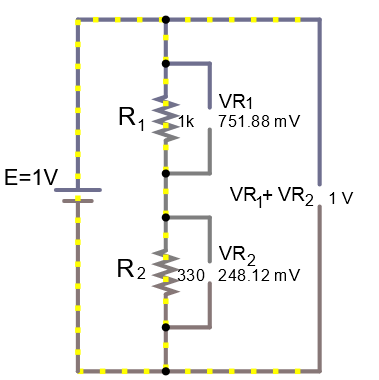
\includegraphics[width=.9\linewidth]{volts_1}
\end{subfigure}
\begin{subfigure}{0.48\textwidth}
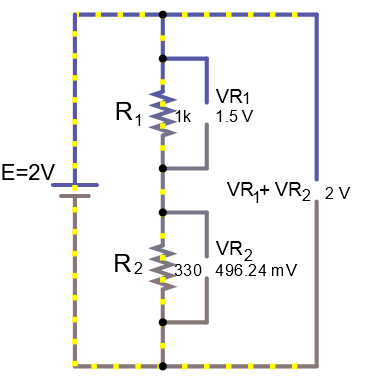
\includegraphics[width=.9\linewidth]{volts_2}
\end{subfigure}
\begin{subfigure}{0.48\textwidth}
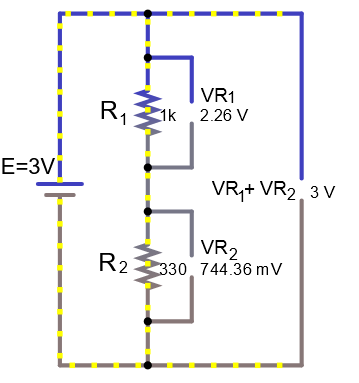
\includegraphics[width=.9\linewidth]{volts_3}
\end{subfigure}
\begin{subfigure}{0.48\textwidth}
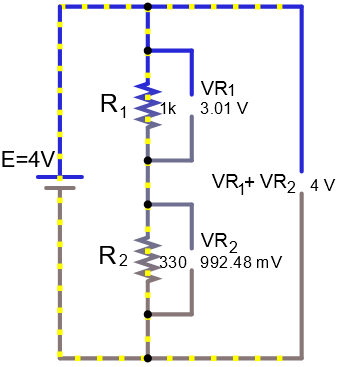
\includegraphics[width=.9	\linewidth]{volts_4}
\end{subfigure}
\caption{Voltmeter simulation for $\SI{1}{\volt}$ to $\SI{4}{\volt}$}
\end{figure}

\begin{figure}
\begin{subfigure}{0.48\textwidth}
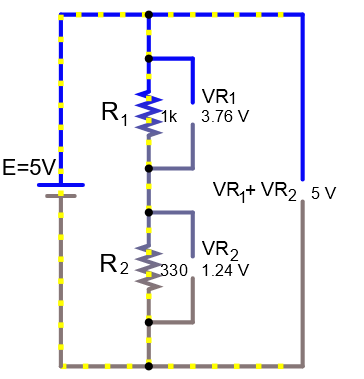
\includegraphics[width=1.03\linewidth]{volts_5}
\end{subfigure}
\begin{subfigure}{0.48\textwidth}
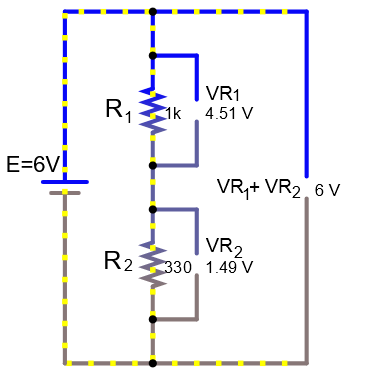
\includegraphics[width=1.03\linewidth]{volts_6}
\end{subfigure}
\begin{subfigure}{0.48\textwidth}
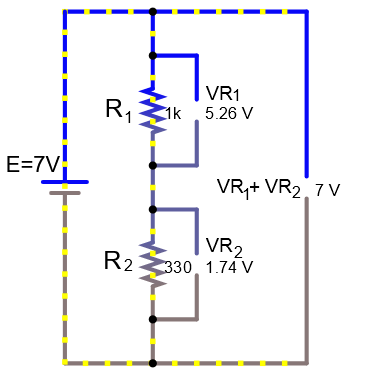
\includegraphics[width=1.03\linewidth]{volts_7}
\end{subfigure}
\begin{subfigure}{0.48\textwidth}
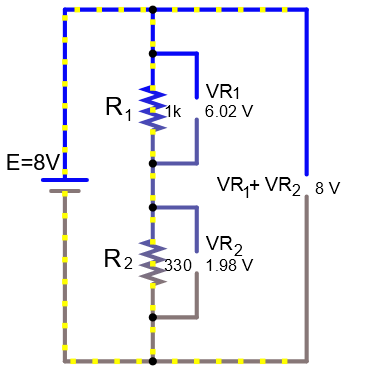
\includegraphics[width=1.03\linewidth]{volts_8}
\end{subfigure}
\begin{subfigure}{0.48\textwidth}
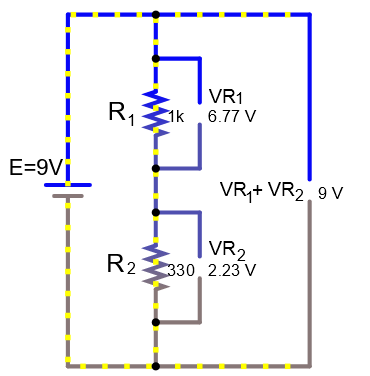
\includegraphics[width=1.03\linewidth]{volts_9}
\end{subfigure}
\begin{subfigure}{0.48\textwidth}
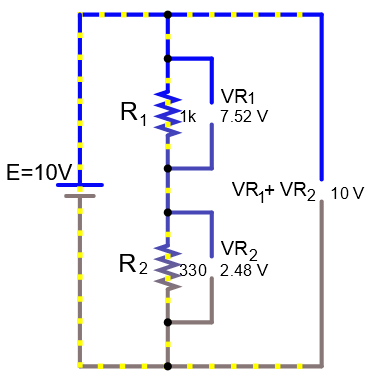
\includegraphics[width=1.03\linewidth]{volts_10}
\end{subfigure}
\caption{Voltmeter simulation for $\SI{5}{\volt}$ to $\SI{10}{\volt}$}
\end{figure}
\begin{figure}[H]
\begin{subfigure}{0.48\textwidth}
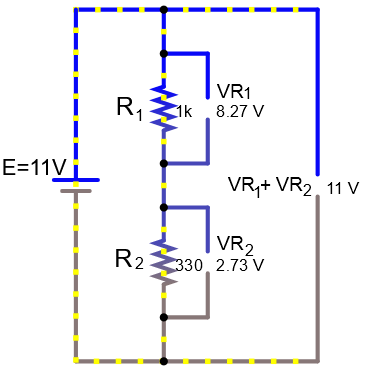
\includegraphics[width=1.05\linewidth]{volts_11}
\end{subfigure}
\begin{subfigure}{0.48\textwidth}
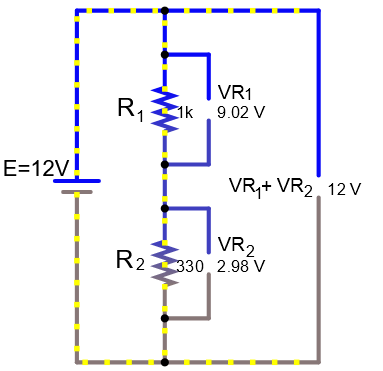
\includegraphics[width=1.05\linewidth]{volts_12}
\end{subfigure}
\caption{Voltmeter simulation for $\SI{11}{\volt}$ and $\SI{12}{\volt}$}
\label{fig:3}
\end{figure}
\subsection{Ammeter usage}
In the last part we used the $\SI{560}{\ohm}$ and $\SI{680}{\ohm}$ resistors to measure current in all the resistors and in the equivalent resistor, augmenting the value of the voltage supply in the same way as the previous part.
\subsubsection{Calculations}
If the resistors are connected in series, each one receives the same voltage supplied by $E$ but the current flowing through them is different and is given, using Ohm's law, by:
\begin{align*}
I_1&=\frac{V}{R_1}\\
I_2&=\frac{V}{R_2}
\end{align*}
Then, the current in the equivalent resistor is given by:
\[I_t=\frac{V}{R_{eq}}\]
Where Req is given by:
\begin{align*}
R_{eq}&=\frac{1}{\frac{1}{R_1}\frac{1}{R_2}}\\
R_{eq}&=\Big(\frac{R_1+R_2}{R_1 R_2}\Big)^{-1}\\
R_{eq}&=\frac{R_1R_2}{R_1+R_2}
\end{align*}
Finally, 
\[I_t=V\cdot\Big(\frac{R_1+R_2}{R_1\cdot_2}\Big)\]
Then, for each voltage we have:\\
%1V
$E=\SI{1}{\volt}$
\[I_1=\frac{\SI{1}{\volt}}{\SI{560}{\ohm}}=\SI{1.786}{\milli\ampere}
\quad
I_2=\frac{\SI{1}{\volt}}{\SI{680}{\ohm}}=\SI{1.470}{\milli\ampere}
\quad
I_{t}=\SI{1}{\volt}\cdot\Big(\frac{\SI{680}{\ohm}+\SI{560}{\ohm}}{\SI{1}{\ohm}\cdot\SI{560}{\ohm}}\Big)=\SI{3.256}{\milli\ampere}
\]
%2V
$E=\SI{2}{\volt}$
\[I_1=\frac{\SI{2}{\volt}}{\SI{560}{\ohm}}=\SI{3.571}{\milli\ampere}
\quad
I_2=\frac{\SI{2}{\volt}}{\SI{680}{\ohm}}=\SI{2.941}{\milli\ampere}
\quad
I_{t}=\SI{2}{\volt}\cdot\Big(\frac{\SI{680}{\ohm}+\SI{560}{\ohm}}{\SI{1}{\ohm}\cdot\SI{560}{\ohm}}\Big)=\SI{6.513}{\milli\ampere}
\]
%3V
$E=\SI{3}{\volt}$
\[I_1=\frac{\SI{3}{\volt}}{\SI{560}{\ohm}}=\SI{5.357}{\milli\ampere}
\quad
I_2=\frac{\SI{3}{\volt}}{\SI{680}{\ohm}}=\SI{4.412}{\milli\ampere}
\quad
I_{t}=\SI{3}{\volt}\cdot\Big(\frac{\SI{680}{\ohm}+\SI{560}{\ohm}}{\SI{1}{\ohm}\cdot\SI{560}{\ohm}}\Big)=\SI{9.769}{\milli\ampere}
\]
%4V
$E=\SI{4}{\volt}$
\[I_1=\frac{\SI{4}{\volt}}{\SI{560}{\ohm}}=\SI{7.143}{\milli\ampere}
\quad
I_2=\frac{\SI{4}{\volt}}{\SI{680}{\ohm}}=\SI{5.882}{\milli\ampere}
\quad
I_{t}=\SI{4}{\volt}\cdot\Big(\frac{\SI{680}{\ohm}+\SI{560}{\ohm}}{\SI{1}{\ohm}\cdot\SI{560}{\ohm}}\Big)=\SI{13.025}{\milli\ampere}
\]
%5V
$E=\SI{5}{\volt}$
\[I_1=\frac{\SI{5}{\volt}}{\SI{560}{\ohm}}=\SI{8.928}{\milli\ampere}
\quad
I_2=\frac{\SI{5}{\volt}}{\SI{680}{\ohm}}=\SI{7.353}{\milli\ampere}
\quad
I_{t}=\SI{5}{\volt}\cdot\Big(\frac{\SI{680}{\ohm}+\SI{560}{\ohm}}{\SI{1}{\ohm}\cdot\SI{560}{\ohm}}\Big)=\SI{16.281}{\milli\ampere}
\]
%6V
$E=\SI{6}{\volt}$
\[I_1=\frac{\SI{6}{\volt}}{\SI{560}{\ohm}}=\SI{10.714}{\milli\ampere}
\quad
I_2=\frac{\SI{6}{\volt}}{\SI{680}{\ohm}}=\SI{8.823}{\milli\ampere}
\quad
I_{t}=\SI{6}{\volt}\cdot\Big(\frac{\SI{680}{\ohm}+\SI{560}{\ohm}}{\SI{1}{\ohm}\cdot\SI{560}{\ohm}}\Big)=\SI{19.538}{\milli\ampere}
\]
%7V
$E=\SI{7}{\volt}$
\[I_1=\frac{\SI{7}{\volt}}{\SI{560}{\ohm}}=\SI{12.5}{\milli\ampere}
\quad
I_2=\frac{\SI{7}{\volt}}{\SI{680}{\ohm}}=\SI{10.294}{\milli\ampere}
\quad
I_{t}=\SI{7}{\volt}\cdot\Big(\frac{\SI{680}{\ohm}+\SI{560}{\ohm}}{\SI{1}{\ohm}\cdot\SI{560}{\ohm}}\Big)=\SI{22.794}{\milli\ampere}
\]
%8V
$E=\SI{8}{\volt}$
\[I_1=\frac{\SI{8}{\volt}}{\SI{560}{\ohm}}=\SI{14.286}{\milli\ampere}
\quad
I_2=\frac{\SI{8}{\volt}}{\SI{680}{\ohm}}=\SI{11.765}{\milli\ampere}
\quad
I_{t}=\SI{8}{\volt}\cdot\Big(\frac{\SI{680}{\ohm}+\SI{560}{\ohm}}{\SI{1}{\ohm}\cdot\SI{560}{\ohm}}\Big)=\SI{26.050}{\milli\ampere}
\]
%9V
$E=\SI{9}{\volt}$
\[I_1=\frac{\SI{9}{\volt}}{\SI{560}{\ohm}}=\SI{16.071}{\milli\ampere}
\quad
I_2=\frac{\SI{9}{\volt}}{\SI{680}{\ohm}}=\SI{13.235}{\milli\ampere}
\quad
I_{t}=\SI{9}{\volt}\cdot\Big(\frac{\SI{680}{\ohm}+\SI{560}{\ohm}}{\SI{1}{\ohm}\cdot\SI{560}{\ohm}}\Big)=\SI{29.307}{\milli\ampere}
\]
%10V
$E=\SI{10}{\volt}$
\[I_1=\frac{\SI{10}{\volt}}{\SI{560}{\ohm}}=\SI{17.857}{\milli\ampere}
\quad
I_2=\frac{\SI{10}{\volt}}{\SI{680}{\ohm}}=\SI{14.706}{\milli\ampere}
\quad
I_{t}=\SI{10}{\volt}\cdot\Big(\frac{\SI{680}{\ohm}+\SI{560}{\ohm}}{\SI{1}{\ohm}\cdot\SI{560}{\ohm}}\Big)=\SI{32.563}{\milli\ampere}
\]
%11V
$E=\SI{11}{\volt}$
\[I_1=\frac{\SI{11}{\volt}}{\SI{560}{\ohm}}=\SI{19.643}{\milli\ampere}
\quad
I_2=\frac{\SI{11}{\volt}}{\SI{680}{\ohm}}=\SI{16.176}{\milli\ampere}
\quad
I_{t}=\SI{11}{\volt}\cdot\Big(\frac{\SI{680}{\ohm}+\SI{560}{\ohm}}{\SI{1}{\ohm}\cdot\SI{560}{\ohm}}\Big)=\SI{35.819}{\milli\ampere}
\]
%12V
$E=\SI{12}{\volt}$
\[I_1=\frac{\SI{12}{\volt}}{\SI{560}{\ohm}}=\SI{21.428}{\milli\ampere}
\quad
I_2=\frac{\SI{12}{\volt}}{\SI{680}{\ohm}}=\SI{17.647}{\milli\ampere}
\quad
I_{t}=\SI{12}{\volt}\cdot\Big(\frac{\SI{680}{\ohm}+\SI{560}{\ohm}}{\SI{1}{\ohm}\cdot\SI{560}{\ohm}}\Big)=\SI{39.076}{\milli\ampere}
\]
\subsubsection{Measurements}
\begin{center}
\begin{tabular}{|c|c|c|c|}
\hline
Voltage & Current - $R_1$ and $R_2$ & Resistor - $R_1$ & Resistor -   $R_2$\\ \hline
$E=\SI{1}{\volt}$ & $\SI{2.640}{\milli\ampere}$ & $\SI{2.150}{\milli\ampere}$ & $\SI{1.100}{\milli\ampere}$ \\ \hline
$E=\SI{2}{\volt}$ & $\SI{5.910}{\milli\ampere}$ & $\SI{3.400}{\milli\ampere}$ & $\SI{2.880}{\milli\ampere}$ \\ \hline
$E=\SI{3}{\volt}$ & $\SI{8.320}{\milli\ampere}$ & $\SI{5.120}{\milli\ampere}$ & $\SI{4.280}{\milli\ampere}$ \\ \hline
$E=\SI{4}{\volt}$ & $\SI{10.580}{\milli\ampere}$ & $\SI{6.820}{\milli\ampere}$ & $\SI{5.670}{\milli\ampere}$ \\ \hline
$E=\SI{5}{\volt}$ & $\SI{15.160}{\milli\ampere}$ & $\SI{8.530}{\milli\ampere}$ & $\SI{7.170}{\milli\ampere}$ \\ \hline
$E=\SI{6}{\volt}$ & $\SI{19.150}{\milli\ampere}$ & $\SI{10.190}{\milli\ampere}$ & $\SI{8.210}{\milli\ampere}$ \\ \hline
$E=\SI{7}{\volt}$ & $\SI{21.910}{\milli\ampere}$ & $\SI{12.010}{\milli\ampere}$ & $\SI{9.790}{\milli\ampere}$ \\ \hline
$E=\SI{8}{\volt}$ & $\SI{25.440}{\milli\ampere}$ & $\SI{13.680}{\milli\ampere}$ & $\SI{11.330}{\milli\ampere}$ \\ \hline
$E=\SI{9}{\volt}$ & $\SI{28.630}{\milli\ampere}$ & $\SI{15.490}{\milli\ampere}$ & $\SI{12.690}{\milli\ampere}$ \\ \hline
$E=\SI{10}{\volt}$ & $\SI{32.510}{\milli\ampere}$ & $\SI{17.390}{\milli\ampere}$ & $\SI{14.190}{\milli\ampere}$ \\ \hline
$E=\SI{11}{\volt}$ & $\SI{36.210}{\milli\ampere}$ & $\SI{18.970}{\milli\ampere}$ & $\SI{15.700}{\milli\ampere}$ \\ \hline
$E=\SI{12}{\volt}$ & $\SI{39.410}{\milli\ampere}$ & $\SI{20.790}{\milli\ampere}$ & $\SI{17.190}{\milli\ampere}$ \\ \hline
\end{tabular}
\end{center}
\subsubsection{Simulations}
\begin{figure}[H]
\begin{subfigure}{0.48\textwidth}
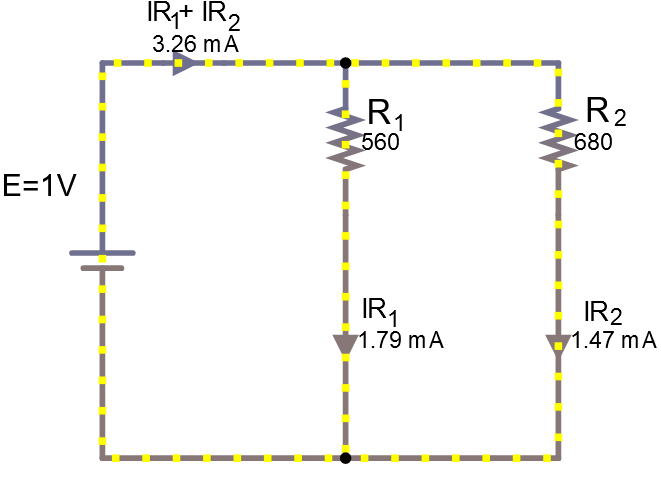
\includegraphics[width=1.16\linewidth]{amps_1}
\end{subfigure}
\begin{subfigure}{0.48\textwidth}
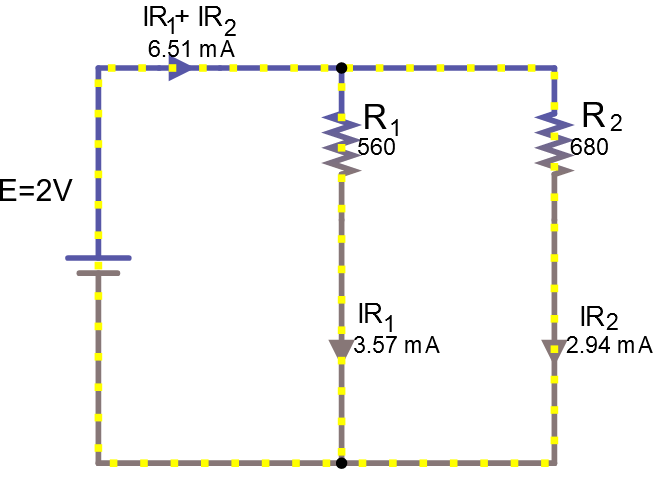
\includegraphics[width=1.16\linewidth]{amps_2}
\end{subfigure}
\begin{subfigure}{0.48\textwidth}
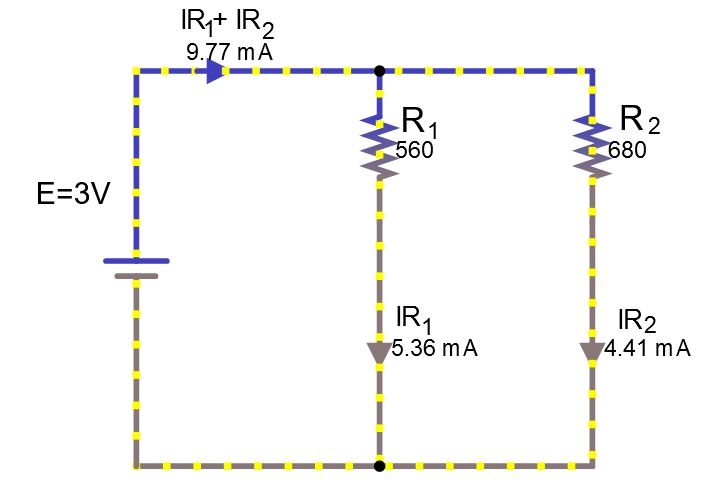
\includegraphics[width=1.16\linewidth]{amps_3}
\end{subfigure}
\begin{subfigure}{0.48\textwidth}
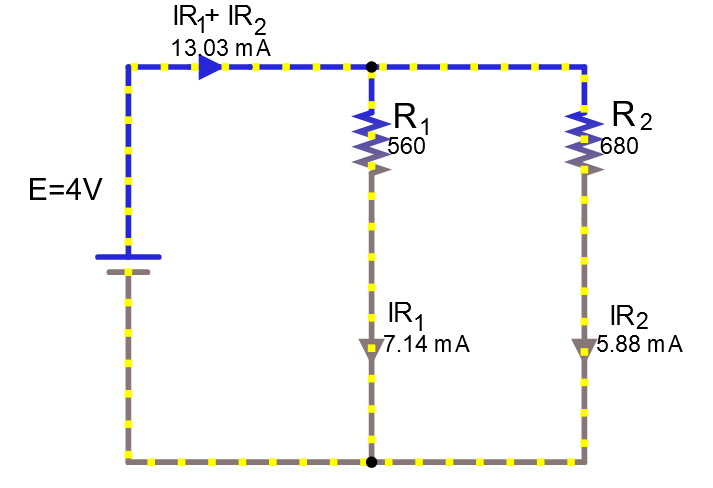
\includegraphics[width=1.16\linewidth]{amps_4}
\end{subfigure}
\begin{subfigure}{0.48\textwidth}
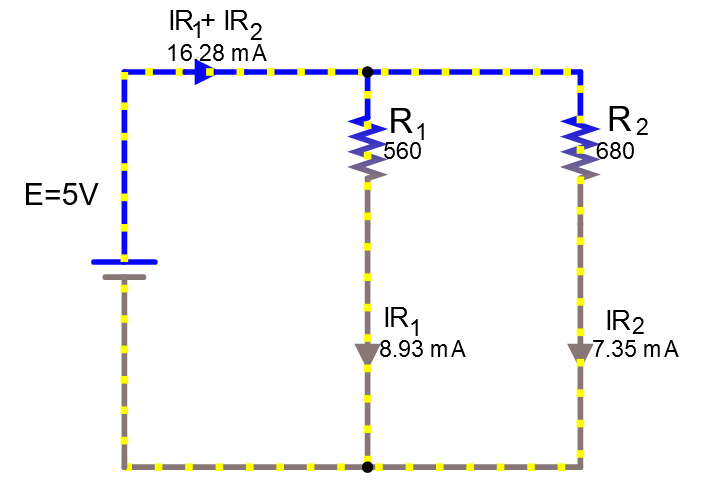
\includegraphics[width=1.16\linewidth]{amps_5}
\end{subfigure}
\begin{subfigure}{0.48\textwidth}
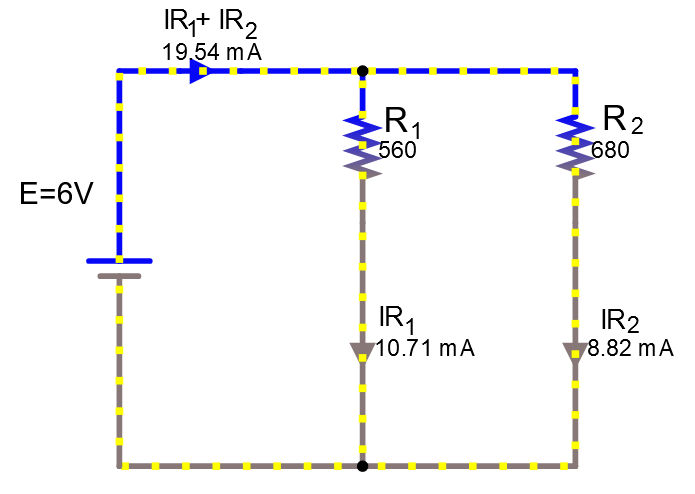
\includegraphics[width=1.16\linewidth]{amps_6}
\end{subfigure}
\caption{Ammeter simulation for $\SI{1}{\volt}$ to $\SI{6}{\volt}$}
\label{fig:4}
\end{figure}

\begin{figure}[H]
\begin{subfigure}{0.48\textwidth}
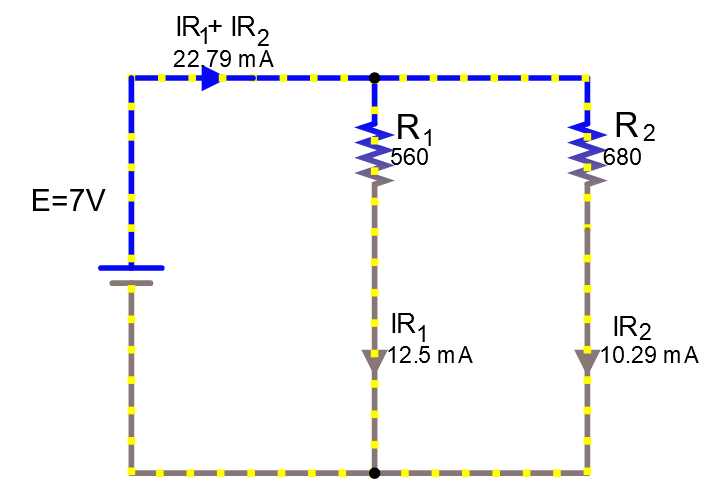
\includegraphics[width=1.16\linewidth]{amps_7}
\end{subfigure}
\begin{subfigure}{0.48\textwidth}
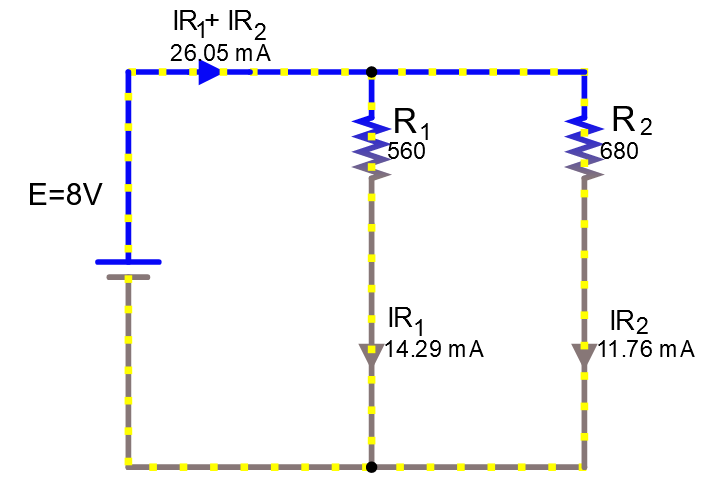
\includegraphics[width=1.16\linewidth]{amps_8}
\end{subfigure}
\begin{subfigure}{0.48\textwidth}
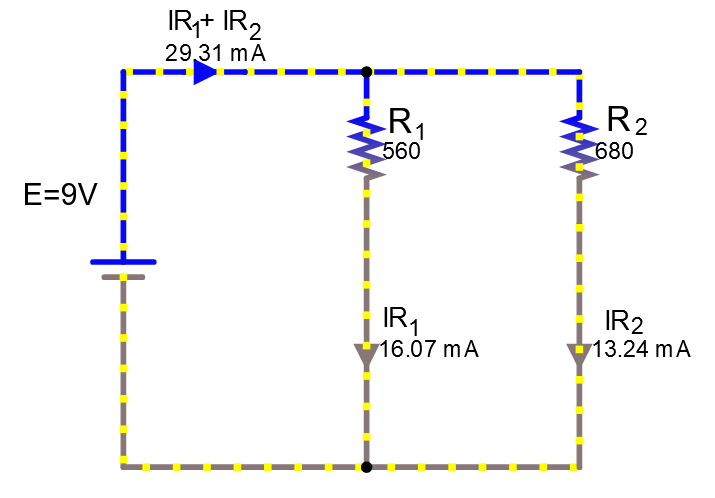
\includegraphics[width=1.16\linewidth]{amps_9}
\end{subfigure}
\begin{subfigure}{0.48\textwidth}
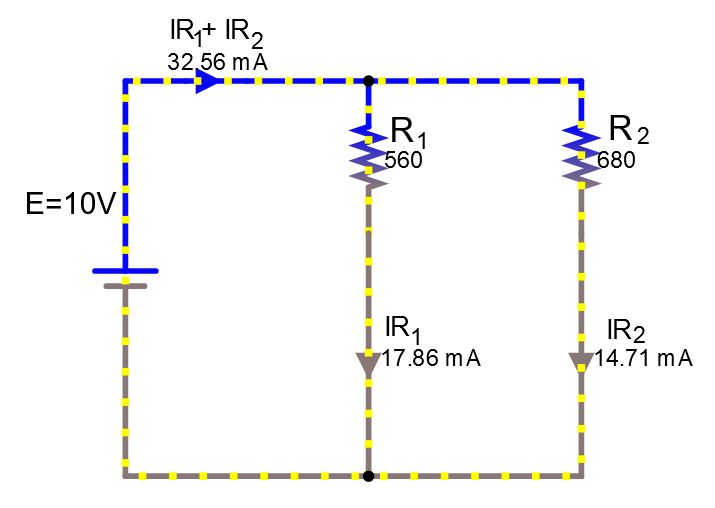
\includegraphics[width=1.16\linewidth]{amps_10}
\end{subfigure}
\begin{subfigure}{0.48\textwidth}
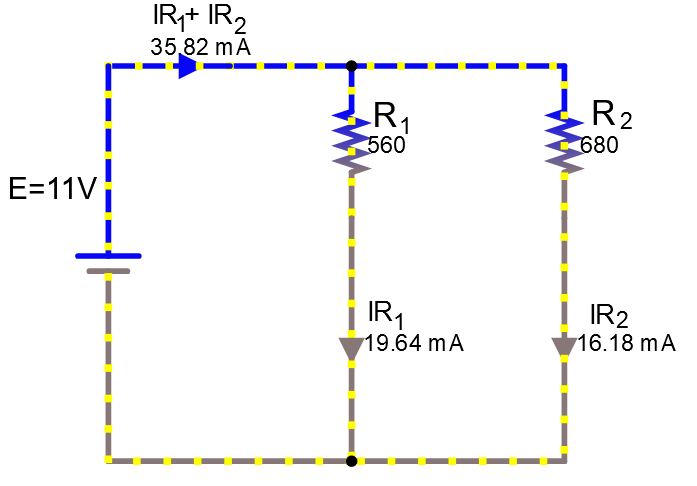
\includegraphics[width=1.16\linewidth]{amps_11}
\end{subfigure}
\begin{subfigure}{0.48\textwidth}
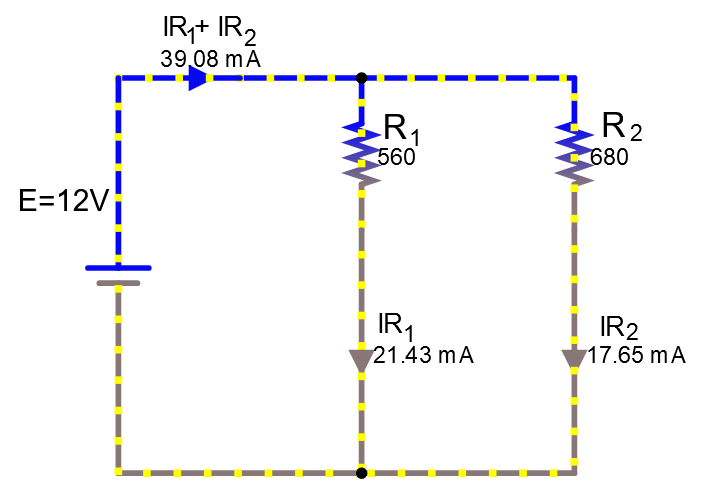
\includegraphics[width=1.16\linewidth]{amps_12}
\end{subfigure}
\caption{Ammeter simulation for $\SI{7}{\volt}$ to $\SI{12}{\volt}$}
\label{fig:5}
\end{figure}
\newpage
\section{Questions}
\textit{What is a series circuit main feature?}\\
When only two elements share a single node, transmitting the same current. 
\textit{What is a parallel circuit main feature?}\\
When two or more elements share a node (non-exclusively). These elements undergo different current values but the same voltage.\\
\textit{What’s the difference between a digital and an analog multimeter?}\\
The analog meter emits sinusoidal pulses and has a needle-like interface, while the digital meter transforms those pulses or signal into a binary format, having also a digital interface.\\
\textit{Why does an ammeter must not be connected in parallel?}\\
Because the ammeter becomes another element in the circuit, and connecting it incorrectly can lead into malfunctioning of the meter or damaging it\\
\textit{Why does a circuit must be de-energized when checking the resistance of an electrical circuit?}\\
Because the current flow would lead to mistakes while trying to measure the resistance. 
\section{Conclusions}
{\large Sabrina:}\\[2ex] 
To practice the correct usage of the multimeter is vital to an engineer’s education, so he or she can monitor every element’s functionality in a circuit, as well as to evaluate their quality. Nevertheless, it is also essential for the student to study well the theoretical part of circuit analysis and construction to have an integral idea to what is really happening in the laboratory\\[2ex] 
{\large Salvador:}\\[2ex]
The evidence shown above shows that the resistances measured had values different from the calculations previously made, but they were approximate values with minimal differences. The correct use of multimeter showed us this minimal differences from calculations and practice\\[2ex]
{\large Sebastián:}\\[2ex]
The experiment helped us to learn the usage of this instruments as well as how they could help us to verify the accuracy of our theoretical designs when they become real world models
\end{document}

